\section{Smooth 0--1 Loss Approximation}
\label{cha:Smoothlossapprox}

The non-smooth, non-differentiable 0--1 loss can be
approximated by a smooth differentiable loss (a modification of sigmoidal loss)
$$l_i = \mathbb{I} [t_i \w^T \xi \leq 0] \approx \frac{1}{1 + e^{Kt_i \w^T \xi }} = \tilde{l}_i^K.$$
This approximation is illustrated by Figure \ref{fig:sla.smooth} (top) for different
values of the \emph{precision constant} $K \in \R^+$ that modulates smoothness.
Assuming the $\xi$ do not lie
on the decision hyperplane, then $\lim_{K \rightarrow +\infty} \tilde{l}_i^K = l_i$.

%%%%%%%%%%%%%%%%%%%%%%%%%%%%%%%%%%%%%%%%%%%%%%%%%%%%%%%%%%
\begin{figure}[tp!]
\hspace{-3mm} 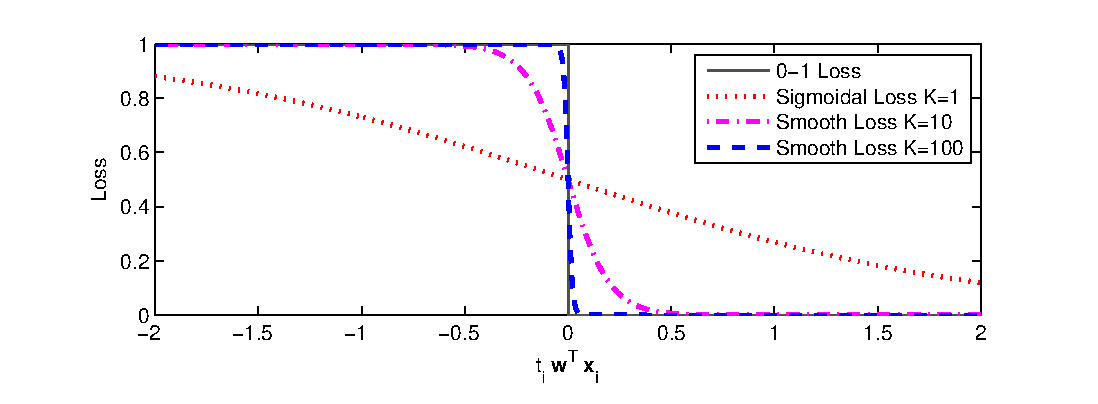
\includegraphics[width=0.50\textwidth]{images/fig52_smooth.eps}
\vspace{-4mm} \hspace{-3mm} 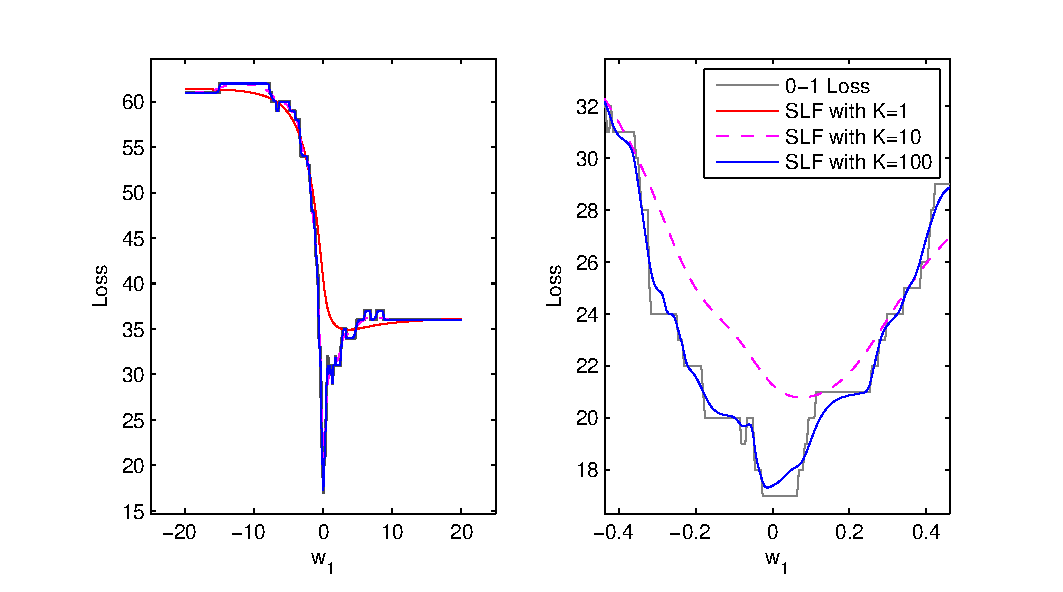
\includegraphics[width=0.50\textwidth]{images/fig53_smoothfunction.eps}
\vspace{-1mm}
\caption{ \footnotesize (top) Sigmoid approximation $\tilde{l}_i^K$ of
  0--1 loss for varying $K$.  (bottom) Comparison of $\sum_{i=1}^N
  \tilde{l}_i^K$ and $\sum_{i=1}^N l_i$ of the 0--1 loss for sample
  data vs. $w_1$ with other components of $\w$ held fixed.  The plot
  on the right is a close-up of the plot on the left around the global
  minimum.}
\label{fig:sla.smooth}
\vspace{-4mm}
\end{figure}
%%%%%%%%%%%%%%%%%%%%%%%%%%%%%%%%%%%%%%%%%%%%%%%%%%%%%%%%%%

Figure \ref{fig:sla.smooth} (bottom) illustrates how an objective
based on $L_K(\w^*) = \sum_{i=1}^N \tilde{l}_i^K$ changes with
different values of the precision constant $K$ w.r.t. the actual 0--1
loss $\sum_{i=1}^N l_i$.  Clearly, small $K$ yields smoother
objectives with few local minima but provide only a rough
approximation of the true objective, while the opposite is true for
large $K$.

This suggests the following iterative unrelaxed optimization approach
for zeroing in on the optimum 0--1 loss value: start with a small
value of $K$ and iteratively increase it; at each iteration with a
fixed $K$, initialize with the solution from the previous iteration
and perform coordinate descent to locally optimize each $w_i$ ($0 \leq
i \leq D$) in turn.  This is summarized in the SLA algorithm 
(Algorithm~\ref{alg:sla.algorithm}).  Of key importance here is the local
search \textsc{Grad-Desc-in-Range} algorithm defined in
Algorithm~\ref{alg:sla.range}.  Because of local optima (that increase
with $K$) this is a mixture of gradient descent, pattern search
methods~\cite{Hooke}, and a hill-climbing heuristic.  In short, this
hybrid local search algorithm iterates between gradient descent to
find a local optima followed by a probed search at uniform intervals
to find potentially better positions, this process repeating until 
an improved solution is found.  Constants that work well in practice
for SLA are the following: $r_R = 2^{-1}, R0 = 8, r_\epsilon = 2^{-1}, 
\epsilon_{S0} = 0.2, r_K = 10, K_{MIN} = 2, \quad K_{MAX} = 200$.

%%%%%%%%%%%%%%%%%%%%%%%%%%%%%%%%%%%%%%%%%%%%%%%%%%%%%%%%%%%%%%%%
\begin{algorithm}
%\vspace{-3mm}
\caption{Smooth 0--1 Loss Approximation (SLA)}
\label{alg:sla.algorithm}
{\footnotesize
\begin{algorithmic}[1]
\INPUT {Training data $(\X,\t)$}
\OUTPUT {Weights $\w^*$ (approx.) minimizing 0--1 loss}
\FUNCTION {{\sc Find-SLA-Solution}($\X, \t$)} %\COMMENT{returns $\w^*$}
   \STATE $\w^* \gets \w^*_{\mathit{SVM}}$ from SVM solution for $(\boldsymbol{X},\t)$
   \STATE $R \gets R0$
   \STATE $\epsilon_S \gets \epsilon_{S0}$
   \STATE $K \gets K_{MIN}$
   \WHILE {$K \leq K_{MAX}$}
      \STATE $\w^* \gets$ {\sc Grad-Desc-in-Range}($\w^*, K, R, \epsilon_S$)
      \STATE $K \gets r_K.K$
      \STATE $R \gets r_R.R$
      \STATE $\epsilon_S \gets r_\epsilon.\epsilon_S$
   \ENDWHILE
   \STATE {\bfseries return} $\w^*$
\ENDFUNCTION
\end{algorithmic}}
%\vspace{-4mm}
\end{algorithm}
%%%%%%%%%%%%%%%%%%%%%%%%%%%%%%%%%%%%%%%%%%%%%%%%%%%%%%%%%%%%%%%%

%%%%%%%%%%%%%%%%%%%%%%%%%%%%%%%%%%%%%%%%%%%%%%%%%%%%%%%%%%%%%%%%%%%%%%
\begin{algorithm}[t!]
%\vspace{-3mm}
\caption{Range Optimization for SLA}
\label{alg:sla.range}
{\footnotesize
\begin{algorithmic}[1]
\INPUT {$\w$, $K$, radius $R$, step size $\epsilon_S$}
\OUTPUT {Approx. optimal solution $\w^*$} 

\FUNCTION{{\sc Grad-Desc-in-Range}($\w, K, R, \epsilon_S$)} 
\REPEAT
   \STATE \COMMENT {{\it Stage 1: Find a local minimum} \hfill$\qquad\qquad$ \;}
   \STATE $\w^* \gets \w$
   \REPEAT
      \STATE $r \gets max_{rate}$
      \STATE $\w \gets (\w^* - r \nabla L_K(\w^*))$
      \WHILE{$(r \!\! \geq \!\! min_{rate}) \!\! \land \!\! (L_K(\!\w^*) \!\! - \!\! L_K(\w) \!\! < \!\! \epsilon_L) $}
         \STATE $r \gets 0.1 r$
         \STATE $\w \gets (\w^* - r\nabla L_K(\w^*))$
      \ENDWHILE
      \IF{$r \geq min_{rate}$}
         \STATE $\w^* \gets \w$
      \ENDIF
   \UNTIL{$(-\epsilon_G \preccurlyeq  \nabla L_K(\w^*) \preccurlyeq \epsilon_G) \lor (r < min_{rate})$}
   \STATE \COMMENT{\it Stage 2: Probe in radius $R$ to escape minimum}
   \FOR {$i=0$ to $D$}
      \FOR {$step \! \in \! \{\epsilon_S,\! -\epsilon_S, 2\epsilon_S,\! -2\epsilon_S, \dots, R, \! -R \}$}
         \STATE $\w \gets \w^*$  
         \STATE $w_i \gets w_i + step$
         \IF{$L_K(\w^*) - L_K(\w) \geq \epsilon_L$}
            \STATE {\bf go to step 3}
         \ENDIF       
      \ENDFOR
   \ENDFOR
\UNTIL{$L_K(\w^*) - L_K(\w) < \epsilon_L$}
\STATE {\bfseries return} $\w^*$
\ENDFUNCTION
\end{algorithmic}}
%\vspace{-4mm}
\end{algorithm}
%%%%%%%%%%%%%%%%%%%%%%%%%%%%%%%%%%%%%%%%%%%%%%%%%%%%%%%%%%%%%%%%%%%%%%

